\documentclass[11pt,a4paper]{article}

\usepackage[utf8]{inputenc}
\usepackage[T1]{fontenc}
\usepackage[french]{babel}
\usepackage{geometry}
\usepackage{graphicx}
\graphicspath{{figures/}}
\usepackage{float}
\usepackage{listings}
\usepackage{hyperref}

\geometry{margin=2.5cm}
\lstset{basicstyle=\ttfamily\small, breaklines=true, frame=single}

% Largeur figures : 100%% si moins de 6 images par TP, sinon 80%%
\newcommand{\setfigw}[1]{%
  \ifnum#1<6
    \def\figw{1.0\linewidth}%
  \else
    \def\figw{0.8\linewidth}%
  \fi
}

\title{\textbf{Compte rendu unifié — Moteur Sentinel}\\[0.3em]
\large Deep Learning Modeling pour l'Ingénieur\\TP1 · TP2 · TP3 · TP4 · TP5 · TP6}
\author{Ronald Tatchemo Guiafaing\\Institut Universitaire de la Côte (IUC)}
\date{\today}

\begin{document}
\maketitle
\tableofcontents
\newpage

%==============================================================================
\part{TP1 — Modèle Simulink et signatures électriques}
%==============================================================================
\setfigw{8}

\section{Ce que j'ai fait}
J'ai ouvert le modèle \texttt{Moteur\_Asynchrone\_Base2019bG.slx} dans Simulink. J'ai lancé les simulations à la main avec le bouton \textbf{Run}, en changeant la position du \texttt{Fault\_Switch} et la fréquence de \texttt{Vibration\_Defaut}.

\section{Blocs principaux (ce que j'ai compris)}
\begin{figure}[H]
  \centering
  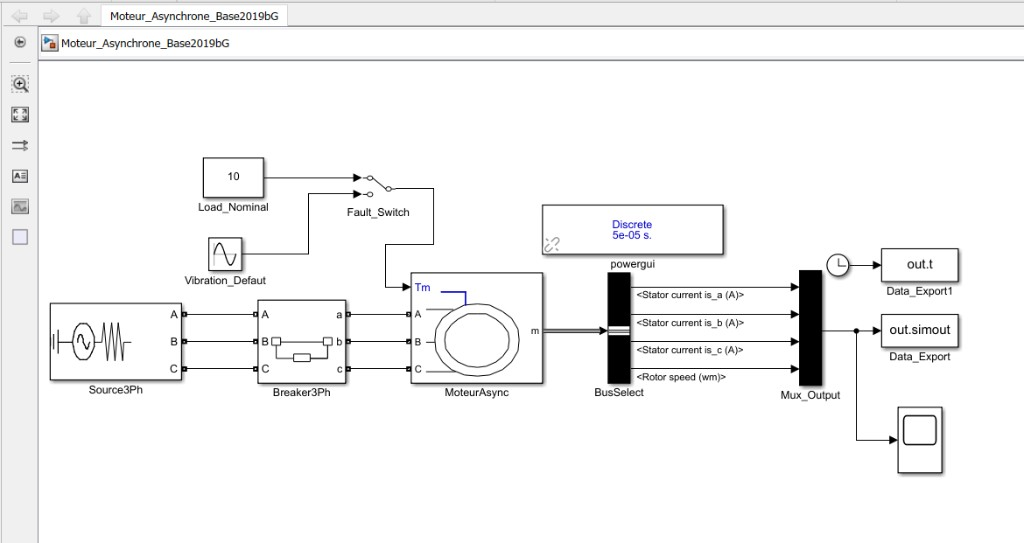
\includegraphics[width=\figw]{Fig00_Schema_Simulink}
  \caption{Schéma Simulink — \texttt{Moteur\_Asynchrone\_Base2019bG.slx}.}
\end{figure}

\begin{itemize}
   \texttt{Source3Ph} : alimentation triphasée 50~Hz, 380~V.
   \texttt{MoteurAsync} : moteur asynchrone (courants + vitesse rotor).
   \texttt{Fault\_Switch} : en haut = moteur sain, en bas = défaut activé.
   \texttt{Vibration\_Defaut} : vibration ajoutée sur le couple (déséquilibre ou roulement).
  \item \texttt{Data\_Export} : enregistre \texttt{simout} (courant phase A, etc.).
\end{itemize}

\section{Réponses Section 3}
\begin{enumerate}
  \item Fréquence source : \textbf{50~Hz}. Tension : \textbf{380~V} (ligne-ligne).
  \item Charge mécanique : bloc \texttt{Load\_Nominal} (10~N·m) + couple de défaut via le switch.
  \item \texttt{BusSelect} : choisit les 4 signaux à afficher (courants + vitesse).
  \item Deux blocs To Workspace : \texttt{simout} (données) et \texttt{t} (temps).
\end{enumerate}

\section{Observations (Section 4 et 5)}
\textbf{Moteur sain :} courant quasi sinusoïdal après le démarrage.

\begin{figure}[H]
  \centering
  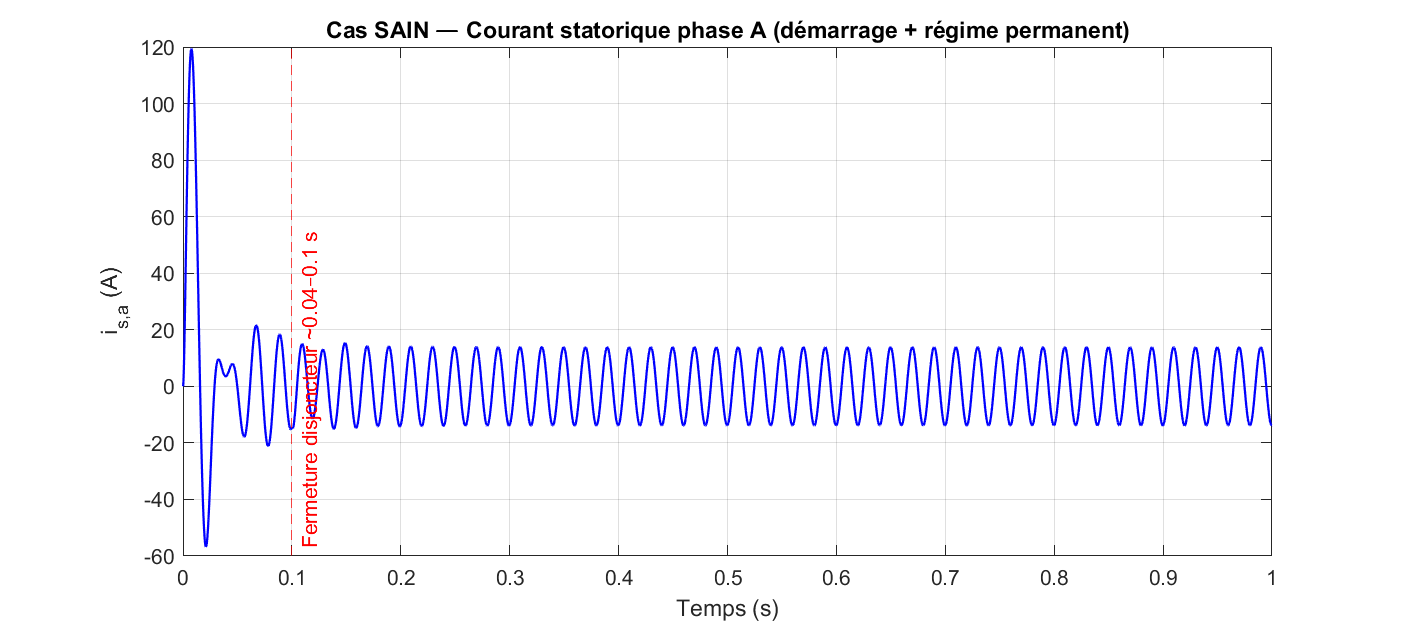
\includegraphics[width=\figw]{Fig01_Courant_Sain_PhaseA.png}
  \caption{Courant phase A — moteur sain (démarrage + régime permanent).}
\end{figure}

Au démarrage, l'appel de courant est très fort (rotor bloqué). En zoom sur les premières 0,25~s :

\begin{figure}[H]
  \centering
  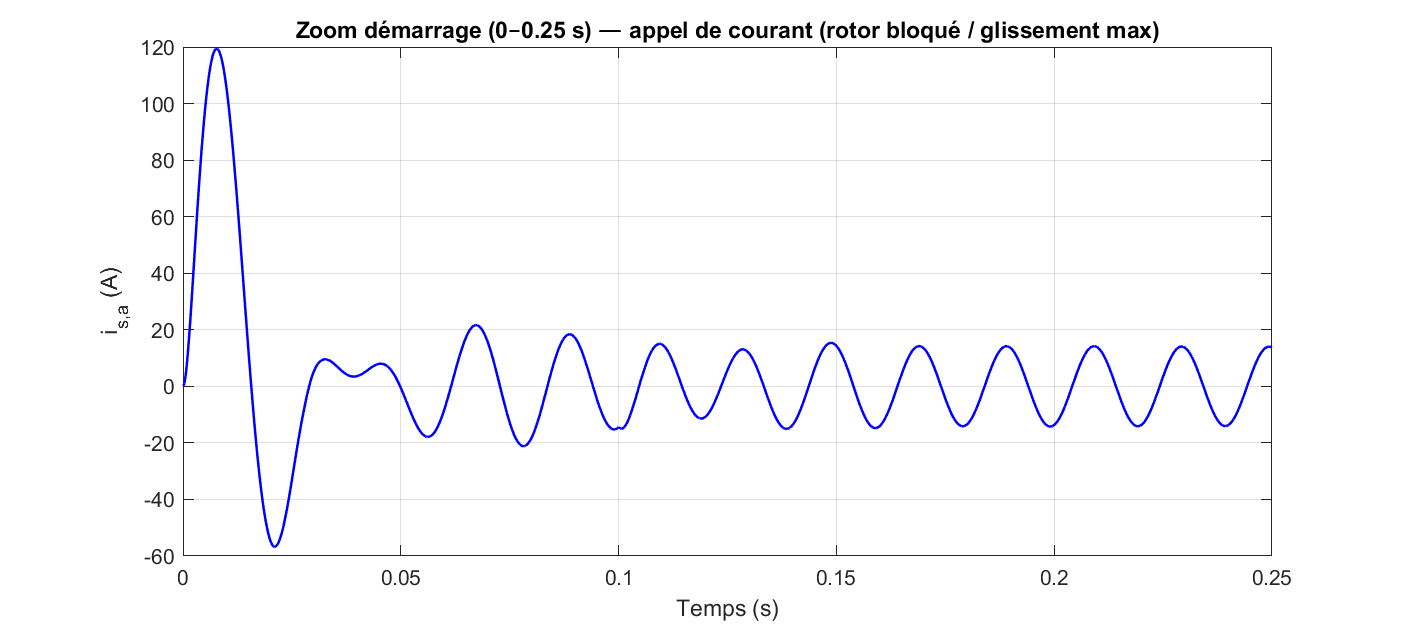
\includegraphics[width=\figw]{Fig02_Demarrage_Zoom.png}
  \caption{Zoom démarrage — pic d'appel de courant.}
\end{figure}

En régime permanent, le courant devient quasi sinusoïdal à 50~Hz :

\begin{figure}[H]
  \centering
  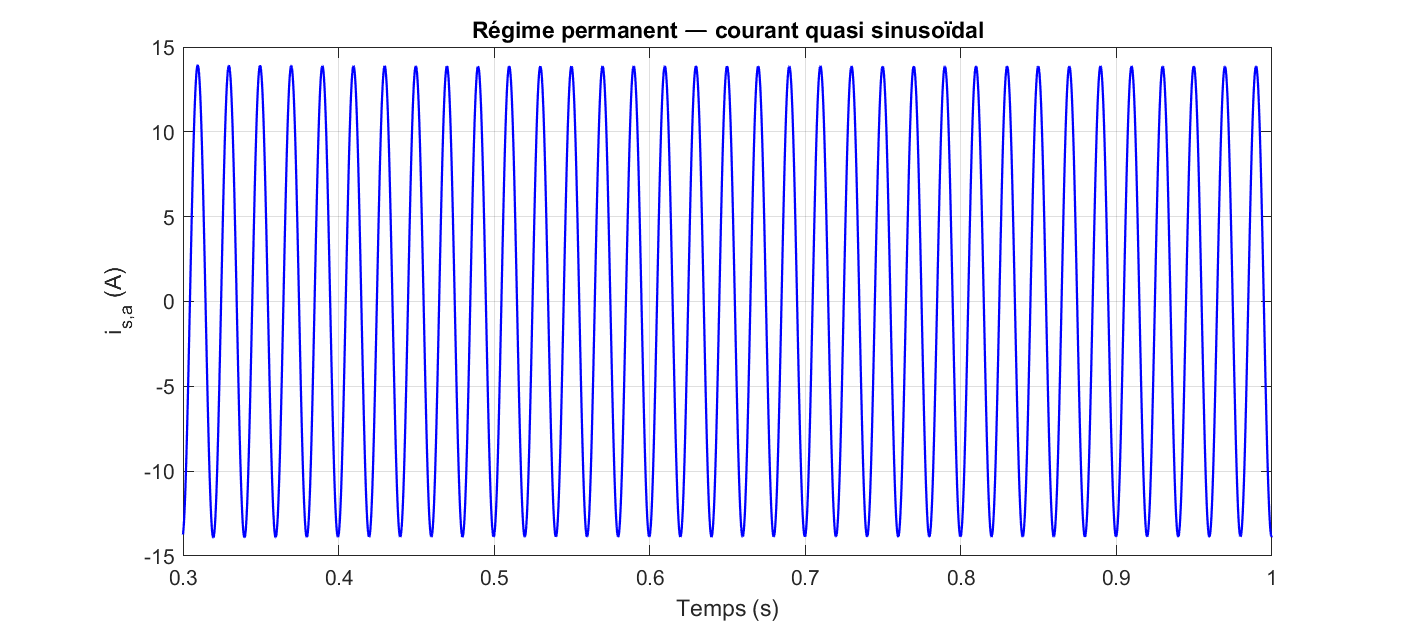
\includegraphics[width=\figw]{Fig03_Regime_Permanent.png}
  \caption{Régime permanent — courant quasi sinusoïdal (0,3--1~s).}
\end{figure}

La vitesse du rotor se stabilise vers une valeur constante :

\begin{figure}[H]
  \centering
  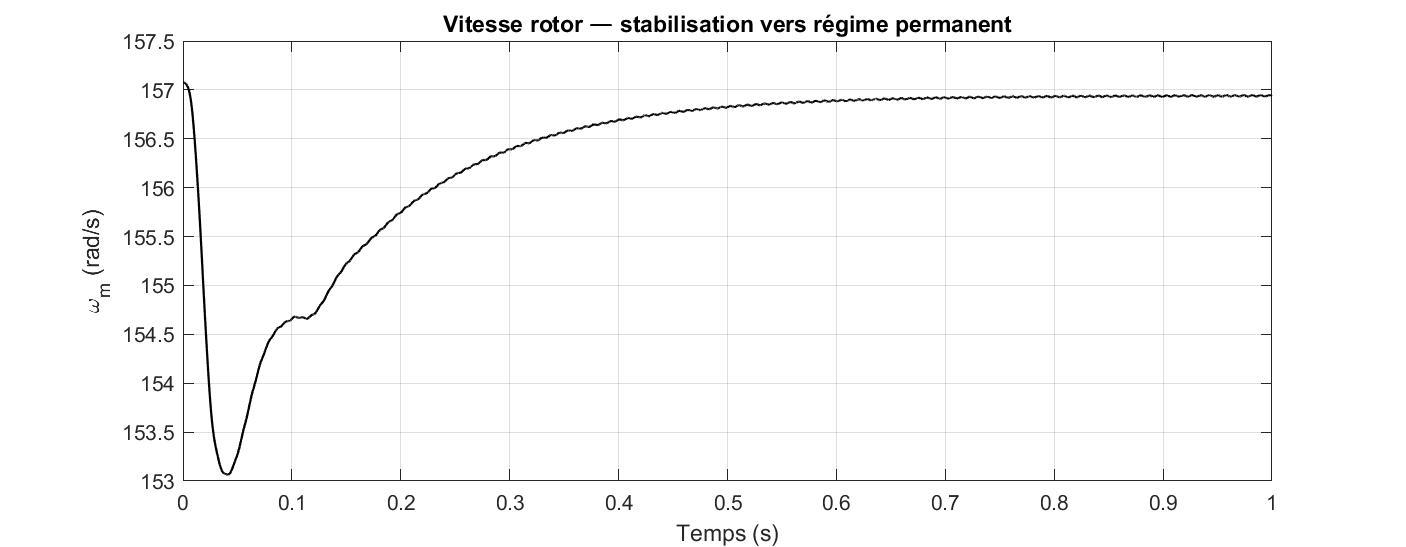
\includegraphics[width=\figw]{Fig04_Vitesse_Rotor_Sain.png}
  \caption{Vitesse rotor $\omega_m$ — stabilisation vers le régime permanent.}
\end{figure}

\textbf{Déséquilibre (157~rad/s) :} l'amplitude du courant n'est plus strictement constante — la différence est surtout visible en FFT (voir figure spectrale ci-dessous).

\textbf{Roulement (800~rad/s) :} sur le Scope, le défaut est difficile à lire à l'œil nu dans le domaine temporel.

\begin{figure}[H]
  \centering
  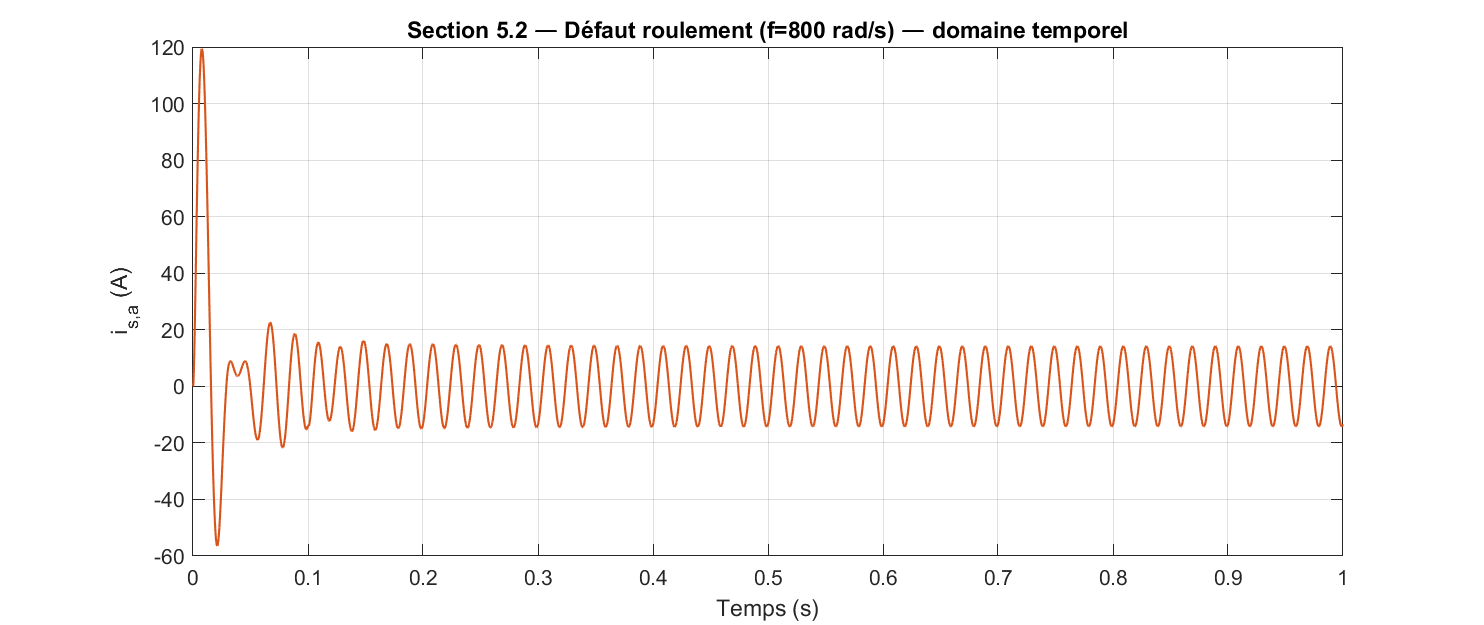
\includegraphics[width=\figw]{Fig07_Bearing_Temporel.png}
  \caption{Défaut roulement — domaine temporel.}
\end{figure}

En fréquence, les défauts deviennent plus parlants. Spectre du roulement et comparaison sain / déséquilibre :

\begin{figure}[H]
  \centering
  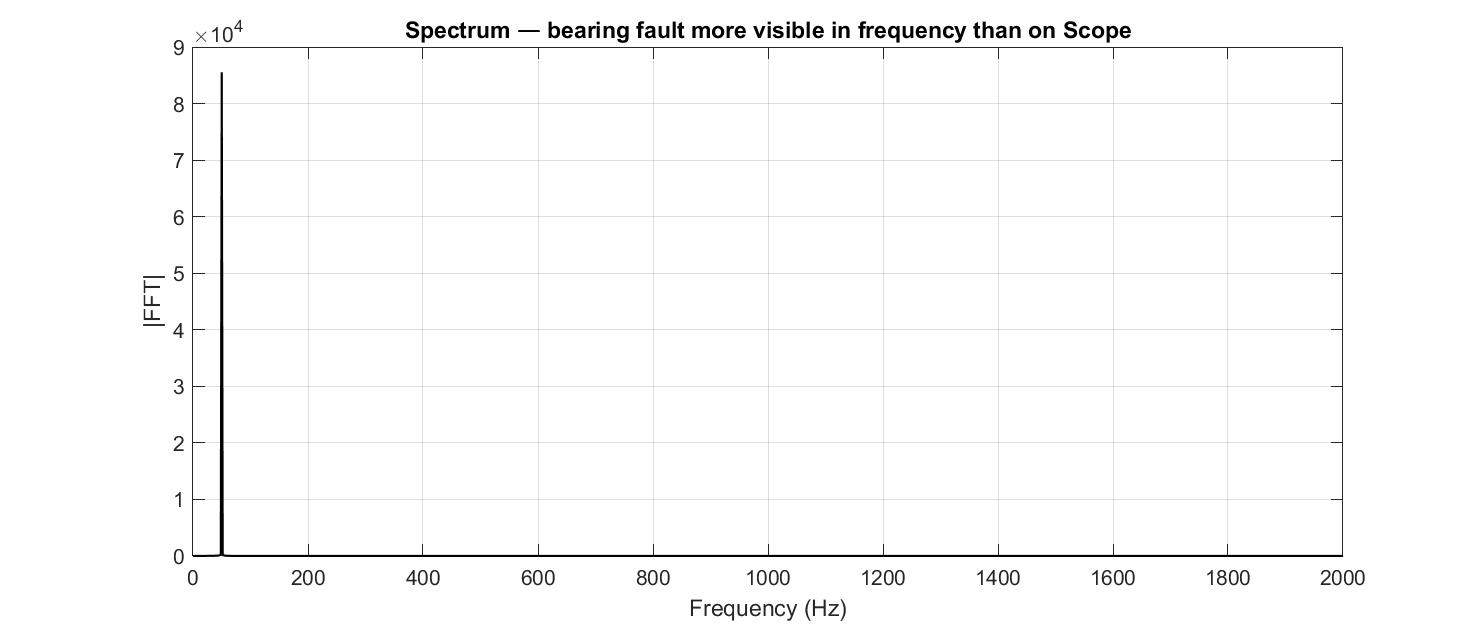
\includegraphics[width=\figw]{Fig09_FFT_Bearing.png}
  \caption{FFT — défaut roulement (pic dominant à 50~Hz).}
\end{figure}

\begin{figure}[H]
  \centering
  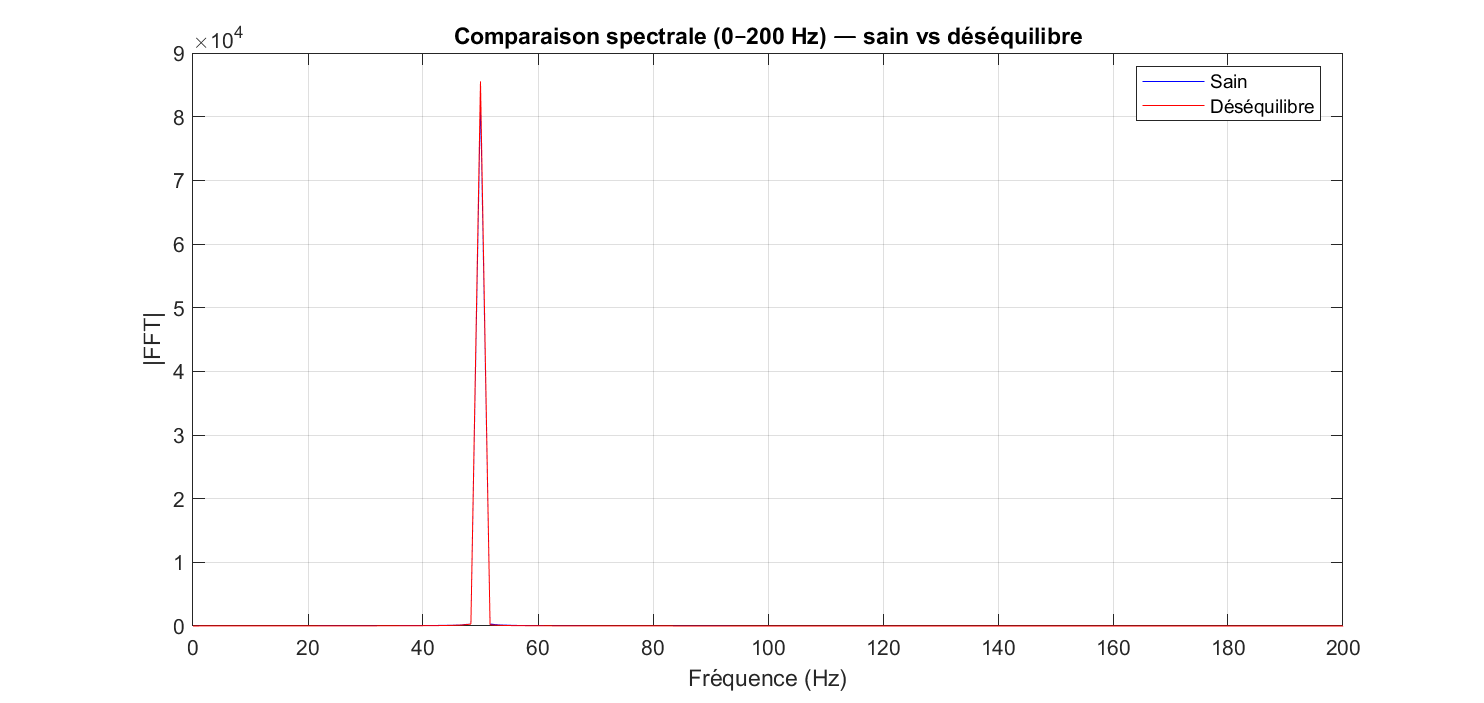
\includegraphics[width=\figw]{Fig10_FFT_Sain_vs_Unbalance.png}
  \caption{Comparaison spectrale 0--200~Hz — sain vs déséquilibre.}
\end{figure}

\section{Question Section 7}
\textbf{Pourquoi le courant statorique renseigne sur l'état mécanique ?}\\
Parce que le couple électromagnétique lie l'électrique et le mécanique. Si le rotor ou la charge est perturbé (déséquilibre, roulement), le courant statorique change aussi. C'est le principe de la MCSA : diagnostiquer la mécanique à partir du courant, sans capteur de vibration sur l'arbre.

%==============================================================================
\part{TP2 — Génération automatisée de données}
%==============================================================================
\setfigw{3}

\section{Scripts utilisés}
\texttt{test\_auto.m} (1 simulation visible) et \texttt{generer\_dataset.m} (3000 simulations, facteur x20).

\section{Comment Simulink tourne sans cliquer sur Run ?}
Quand j'ai lancé \texttt{test\_auto.m}, j'ai vu la fenêtre Simulink s'ouvrir et le \texttt{Fault\_Switch} changer de position tout seul. Concrètement :
\begin{enumerate}
   \texttt{open\_system(...)} ouvre le schéma.
   \texttt{set\_param('.../Fault\_Switch', 'sw', '0')} met le switch en mode sain \textbf{sans cliquer}.
   \texttt{sim(...)} lance la simulation (= bouton Run en code).
   \texttt{simOut.simout.signals.values(:,1)} récupère le courant phase A.
\end{enumerate}
Pour les 3000 échantillons (1000 par classe), \texttt{generer\_dataset.m} fait la même chose en boucle, mais Simulink reste invisible (c'est normal, sinon ce serait trop long à regarder).

\section{Exercice 1 — Réponse à la question du prof}
\textbf{Quelle commande change le switch sans cliquer ?}\\
→ \textbf{\texttt{set\_param}} avec le paramètre \texttt{'sw'} du bloc \texttt{Fault\_Switch}.

\begin{figure}[H]
  \centering
  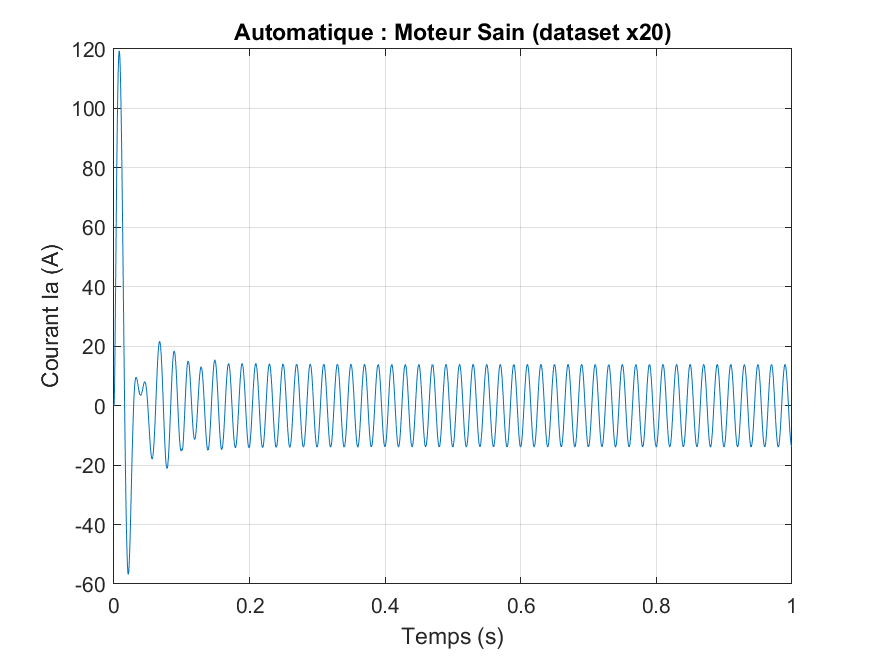
\includegraphics[width=\figw]{TP2_Moteur_Sain.png}
  \caption{Simulation automatique — moteur sain (\texttt{test\_auto.m}).}
\end{figure}

\section{Exercice 2 — Bruit gaussien}
J'ai ajouté du bruit avec \texttt{randn} pour simuler un capteur réel. On voit bien que le signal bruité est plus « sale » que le signal Simulink propre.

\begin{figure}[H]
  \centering
  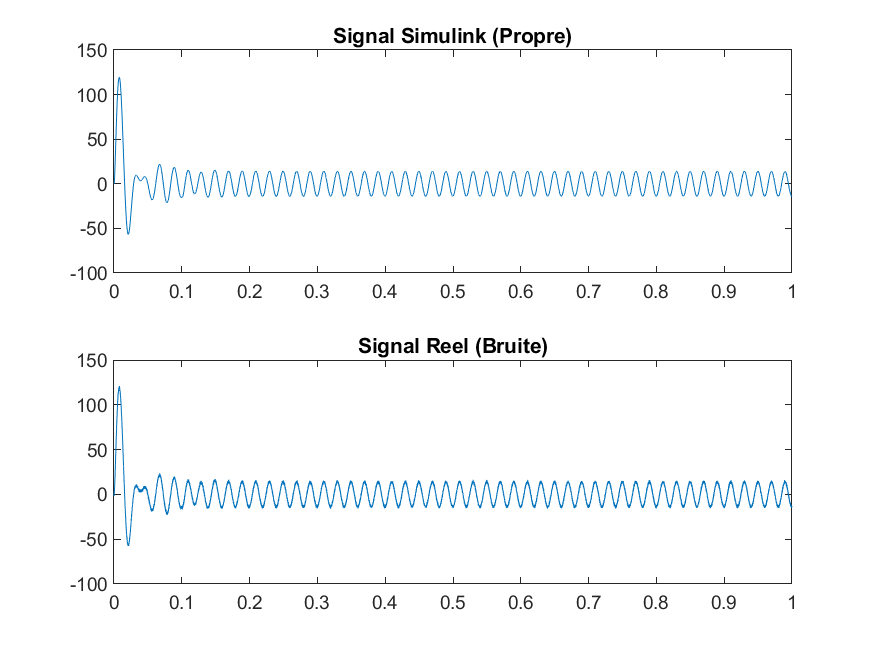
\includegraphics[width=\figw]{TP2_Propre_vs_Bruite.png}
  \caption{Signal propre vs signal bruité.}
\end{figure}

\section{Exercice 3 — Dataset 3000 échantillons}
\texttt{generer\_dataset.m} a tourné environ 15--20 minutes. Résultat :
\begin{itemize}
   50 signaux classe 0 (sain, \texttt{sw=0})
   50 signaux classe 1 (déséquilibre, \texttt{sw=1}, f=157)
   50 signaux classe 2 (roulement, \texttt{sw=1}, f=800~rad/s)
\end{itemize}
Fichier créé : \texttt{data/Dataset\_Moteur.mat}

\section{Exercice 5 — Validation}
J'ai chargé le fichier et vérifié : \texttt{unique(Labels)} donne bien \textbf{[0 1 2]} avec 50 signaux par classe.

\begin{figure}[H]
  \centering
  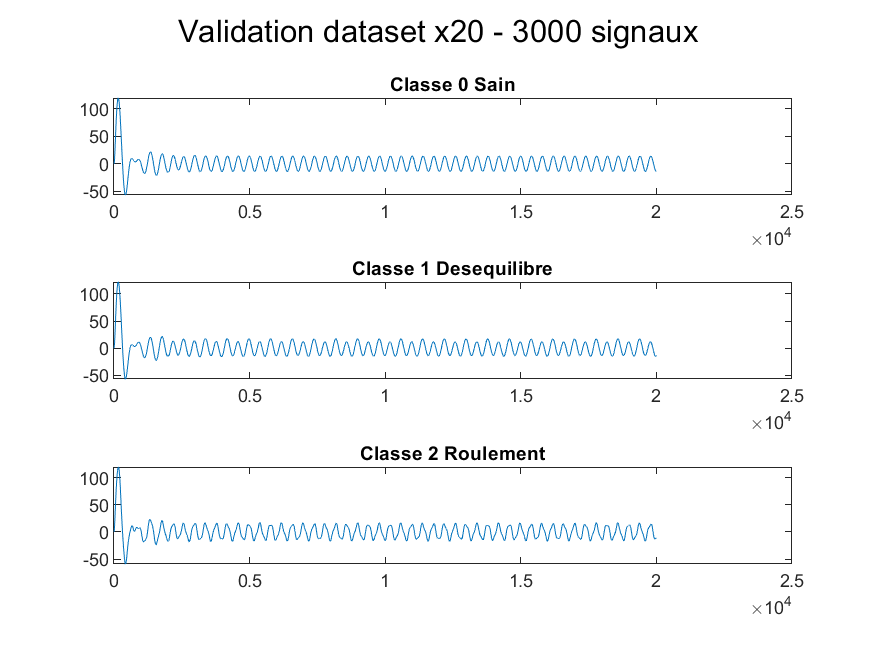
\includegraphics[width=\figw]{TP2_Validation_Dataset.png}
  \caption{Exemples 1, 51 et 101 — une classe par graphique.}
\end{figure}

\section{Question finale (réponse détaillée)}

\textbf{1. Classe 1 vs classe 2 à l'œil nu ?}\\
Non. Quand j'ai tracé l'exemple 51 (déséquilibre) et l'exemple 101 (roulement), les deux courbes se ressemblent beaucoup. Les deux ont des oscillations proches — je n'arrive pas à dire « celui-ci c'est le roulement » juste en regardant le signal dans le temps.

\textbf{2. Un réseau de neurones peut-il le faire sur le signal brut ?}\\
Pas facilement. Si moi je ne vois pas la différence, un MLP qui reçoit 10\,000 points bruts aura le même problème. Par contre, si on transforme le signal en \textbf{spectre} ou \textbf{spectrogramme} (comme au TP3), les défauts apparaissent dans d'autres fréquences autour de 50~Hz — et là un CNN pourra peut-être apprendre des motifs visuels.

\section{Section 6 — Travail personnel (TP2)}
Le prof avait annoncé FFT et spectrogramme. C'est exactement ce qu'on fait au TP3 : passer du signal temporel à une image pour que le CNN puisse « voir » le défaut.

%==============================================================================
\part{TP3 — Du signal physique à l'image}
%==============================================================================
\setfigw{4}

\section{Script}
\texttt{TP3\_Traitement\_Signal.m} — charge \texttt{Dataset\_Moteur.mat} et produit \texttt{Dataset\_Images\_Pret.mat}.

\section{Exercice 1 — Analyse temporelle vs FFT}

\subsection{Rôle de chaque fonction (programme Exercice 1)}
\begin{itemize}
  \texttt{load(...)} : charge \texttt{Dataset} et \texttt{Labels} du TP2.
   \texttt{Dataset\{1\}}, \texttt{Dataset\{101\}} : extrait un signal sain (classe 0) et un signal roulement (classe 2).
   \texttt{Fs = 1/50e-6} : fréquence d'échantillonnage 20~kHz (cohérent avec \texttt{powergui} du modèle).
  \texttt{t = (0:N-1)/Fs} : crée l'axe temps en secondes.
  \texttt{plot(t, signal)} : trace le courant en fonction du temps.
   \texttt{subplot(2,1,...)} : met 2 graphiques l'un sous l'autre dans la même figure.
  \texttt{fft(signal)} : transformée de Fourier — passe du temps aux fréquences.
  \\texttt{abs(...)} : amplitude du spectre (module de la FFT).
  \texttt{f = (0:N-1)*(Fs/N)} : axe des fréquences en Hz.
   \texttt{xlim([0 200])} : zoom sur 0--200~Hz pour voir autour de 50~Hz.
  \texttt{saveas(gcf, ...)} : sauvegarde la figure en PNG.
\end{itemize}

\begin{figure}[H]
  \centering
  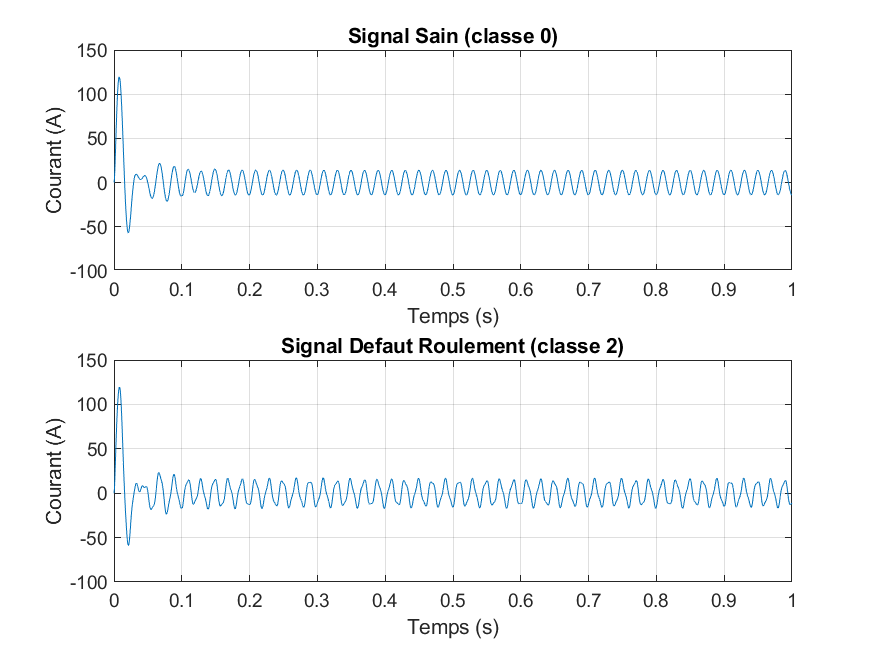
\includegraphics[width=\figw]{TP3_Temporel_Sain_vs_Defaut.png}
  \caption{Domaine temporel — sain vs défaut roulement.}
\end{figure}

\begin{figure}[H]
  \centering
  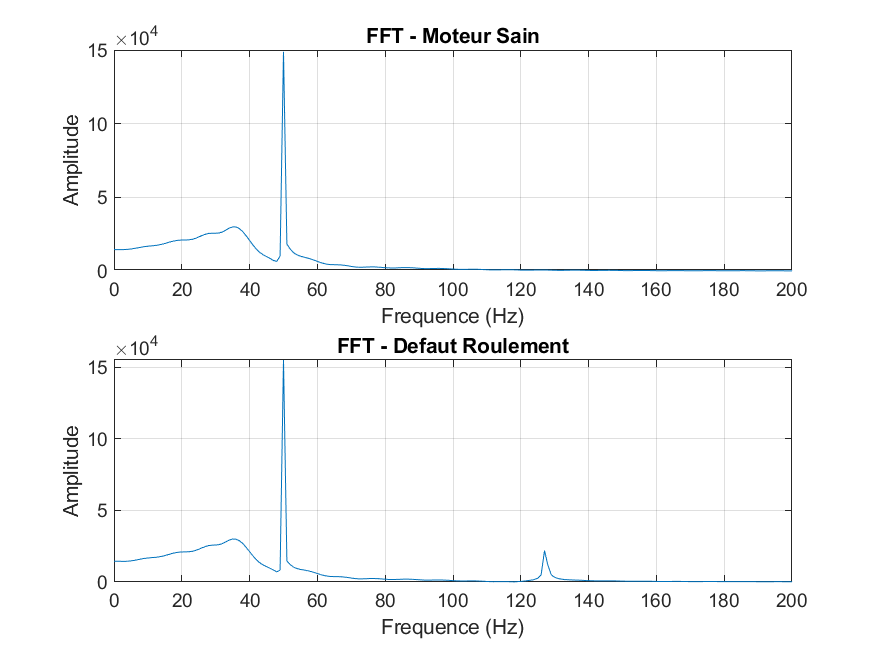
\includegraphics[width=\figw]{TP3_FFT_Sain_vs_Defaut.png}
  \caption{Domaine fréquentiel (FFT) — sain vs défaut roulement.}
\end{figure}

\subsection{Réponses aux questions d'analyse}
\textbf{2. Le défaut est-il clair dans le domaine temporel ?}\\
Non vraiment. Les deux signaux ressemblent à des sinusoïdes modulées. On devine une différence d'amplitude, mais ce n'est pas évident comme sur le Scope du TP1.

\textbf{3. Le défaut est-il plus visible en FFT ?}\\
Oui, plus qu'en temporel. Sur le graphique sain, on voit surtout un pic net à \textbf{50~Hz} (réseau). Sur le graphique défaut, il y a plus d'énergie autour de 50~Hz et des petits pics supplémentaires (harmoniques / bruit) — l'empreinte du défaut est plus lisible en fréquence qu'en temps.

\section{Exercice 2 — Spectrogrammes}

\subsection{Rôle de chaque fonction}
\begin{itemize}
  \item \texttt{pspectrum(signal, Fs, 'spectrogram')} : calcule le spectrogramme (fréquence × temps × intensité). C'est une STFT : on garde \textbf{quand} ET \textbf{quelle fréquence}.
  \item \texttt{10*log10(S + eps)} puis \texttt{mat2gray(...)} : passe en dB avant normalisation (sinon un seul pic domine et l'image devient noire).
  \item \texttt{imresize(..., [227 227])} : redimensionne à 227×227 pixels (taille standard pour AlexNet et autres CNN).
  \item \texttt{imagesc(img)} : affiche la matrice comme une carte de couleurs (heatmap).
   \texttt{colormap jet} : couleurs bleu → rouge selon l'intensité.
  \texttt{colorbar} : barre d'échelle des intensités.
   \texttt{subplot(1,2,...)} : deux spectrogrammes côte à côte pour comparer.
\end{itemize}

\begin{figure}[H]
  \centering
  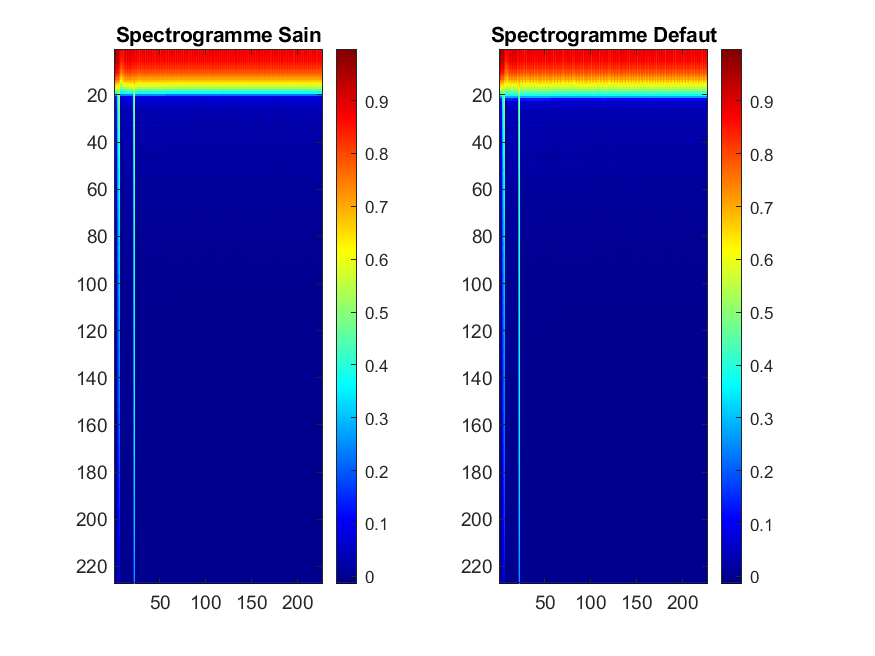
\includegraphics[width=\figw]{TP3_Spectrogrammes_Sain_vs_Defaut.png}
  \caption{Spectrogrammes — sain vs défaut (images 227×227).}
\end{figure}

\subsection{Observation — patterns géométriques ?}
Oui. On ne voit plus une courbe, mais une \textbf{image} avec des bandes horizontales (fréquences fixes) et des zones plus claires ou plus foncées. Un CNN peut apprendre ces motifs (lignes, taches, textures) comme il apprendrait des formes sur une photo — c'est l'idée du cours : transformer un problème électrique en problème de vision.

\section{Exercice 3 — Boucle sur 3000 signaux}

\subsection{Rôle de chaque fonction}
\begin{itemize}
  \item \texttt{numSignals = length(Dataset)} : nombre total d'échantillons (3000).
  \item \texttt{zeros(imgSize, imgSize, 3, numSignals, 'uint8')} : pré-alloue un tableau 4D (hauteur × largeur × 3 canaux RGB × nombre d'images).
  \item \texttt{for i = 1:numSignals} : boucle sur chaque signal.
  \item \texttt{Dataset\{i\}} : récupère le signal numéro \texttt{i}.
  \item \texttt{cat(3, img, img, img)} : copie l'image grise sur 3 canaux → image RGB « fausse couleur » (obligatoire pour les CNN pré-entraînés).
  \item \texttt{im2uint8(...)} : convertit les valeurs 0--1 en entiers 0--255.
  \item \texttt{imgArray(:,:,:,i) = imgRGB} : stocke l'image \texttt{i} dans le tableau géant.
\end{itemize}

\section{Section 6 — Training set (80\% / 20\%)}

\subsection{Rôle de chaque fonction}
\begin{itemize}
  \item \texttt{categorical(Labels, [0,1,2], classes)} : transforme les numéros 0/1/2 en texte « Sain », « Desequilibre », « Roulement ».
  \item \texttt{cvpartition(Y, 'HoldOut', 0.2)} : sépare 80\% train et 20\% validation au hasard (mais équilibré par classe).
  \item \texttt{training(cv)} / \texttt{test(cv)} : indices des échantillons train et validation.
  \item \texttt{XTrain}, \texttt{YTrain}, \texttt{XVal}, \texttt{YVal} : images et labels pour entraîner et tester le réseau au prochain TP.
  \item \texttt{save('Dataset\_Images\_Pret.mat', ...)} : sauvegarde tout pour le CNN (séance 6).
\end{itemize}

Résultat : \textbf{2400 images} en entraînement, \textbf{600} en validation (split 80/20, dataset x20). en entraînement, \textbf{20\%} soit \textbf{30} en validation (split 80/20 via \texttt{cvpartition}).

\begin{figure}[H]
  \centering
  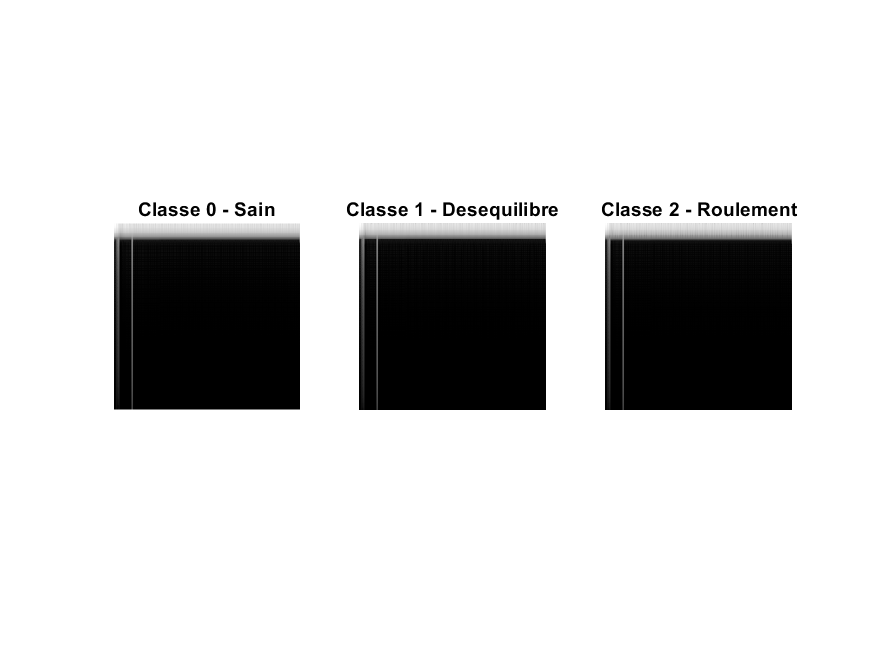
\includegraphics[width=\figw]{TP3_Apercu_3_Classes.png}
  \caption{Aperçu — une image spectrogramme par classe (0, 1, 2).}
\end{figure}

\section{Conclusion TP3}
\begin{itemize}
  \item On est passé d'un \textbf{problème de physique} (courant en Ampères vs temps) à un \textbf{problème de vision} (reconnaissance de motifs sur image).
  \item La FFT seule perd l'information temporelle ; le \textbf{spectrogramme} garde les deux.
   Le fichier \texttt{Dataset\_Images\_Pret.mat} est prêt pour le CNN (séance 6).
\end{itemize}

%==============================================================================
\part{TP4 — Feature Engineering}
%==============================================================================
\setfigw{4}

\section{Script}
\texttt{TP4\_Feature\_Engineering.m} — charge \texttt{Dataset\_Moteur.mat}, extrait 3 indicateurs par signal, normalise (Z-Score) et encode les labels (One-Hot). Produit \texttt{Dataset\_Features\_Pret.mat} pour le MLP (séance 5).

\section{Exercice 1 — RMS, Kurtosis, Peak}
Pour chaque signal du \texttt{Dataset} (signal brut complet) :
\begin{itemize}
   \textbf{RMS} : \texttt{sqrt(mean(signal.\^{}2))} — énergie.
  \textbf{Kurtosis} : \texttt{kurtosis(signal)} — kurtosis d'excès MATLAB (loi normale $\rightarrow$ 0), sensible aux chocs.
  \textbf{Peak} : \texttt{max(abs(signal))} — crête absolue.
\end{itemize}
Stockage : \texttt{Features(i,:) = [val\_rms, val\_kurt, val\_peak]} et \texttt{Labels\_num(i) = Labels(i)}.

\section{Exercice 2 — Visualisation des clusters}
J'utilise \texttt{gscatter} pour tracer RMS (colonne 1) vs Kurtosis (colonne 2), coloré par classe — comme sur la fiche TP4.

\begin{figure}[H]
  \centering
  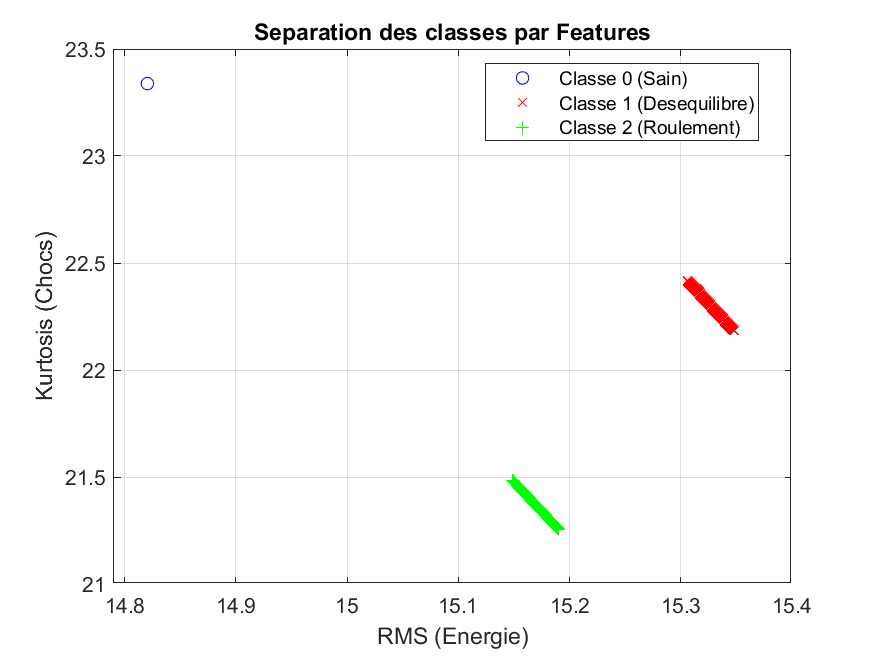
\includegraphics[width=\figw]{TP4_Separation_Classes.png}
  \caption{Séparation des classes par features (RMS vs Kurtosis) — \texttt{gscatter}, marqueurs \texttt{ox+}.}
\end{figure}

\textbf{Figure \texttt{TP4\_Separation\_Classes} :} c'est le graphique principal de la fiche. La classe 0 (sain, bleu) se trouve en haut à gauche avec un Kurtosis plus élevé. Les classes 1 et 2 (rouge et vert) forment un nuage commun en bas à droite : elles ont un RMS plus fort et un Kurtosis plus faible que le moteur sain.

\begin{figure}[H]
  \centering
  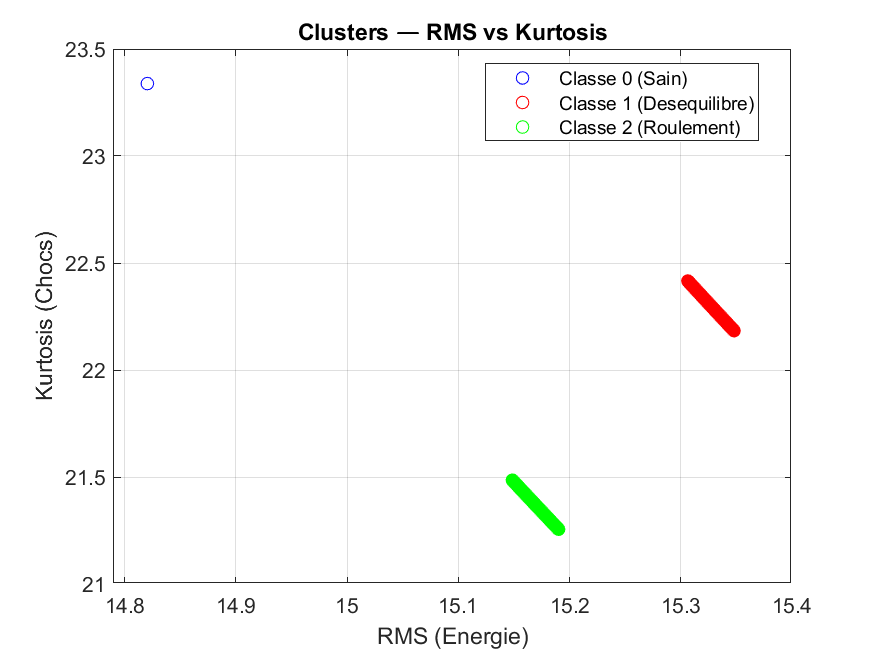
\includegraphics[width=\figw]{TP4_Clusters_RMS_Kurtosis.png}
  \caption{Clusters RMS vs Kurtosis.}
\end{figure}

\textbf{Figure \texttt{TP4\_Clusters\_RMS\_Kurtosis} :} même axe que la figure précédente, avec des marqueurs ronds. On confirme que le \textbf{Kurtosis} est l'indicateur le plus discriminant pour repérer le moteur sain (éloigné du groupe des défauts).

\begin{figure}[H]
  \centering
  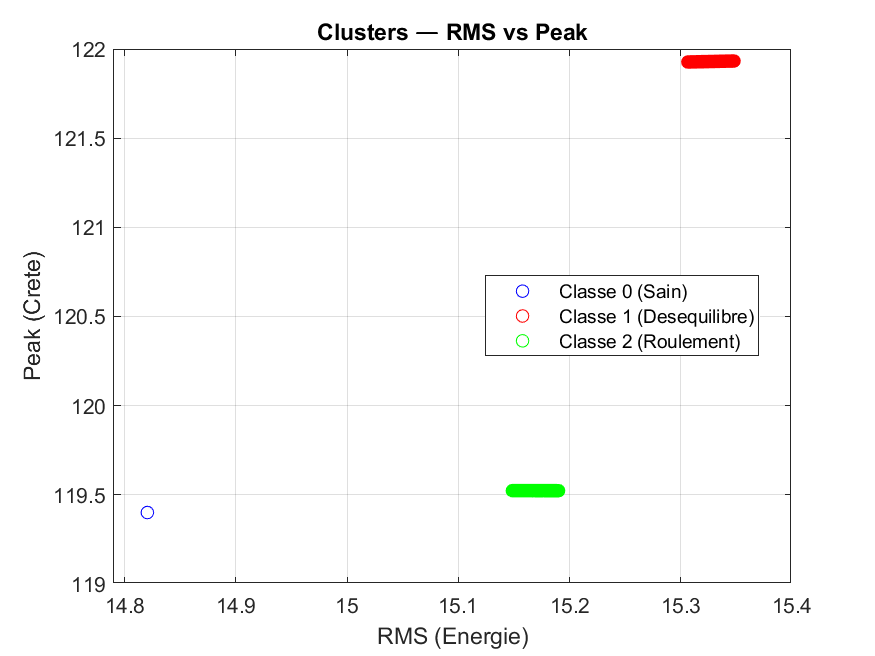
\includegraphics[width=\figw]{TP4_Clusters_RMS_Peak.png}
  \caption{Clusters RMS vs Peak — la crête absolue complète l'analyse.}
\end{figure}

\textbf{Figure \texttt{TP4\_Clusters\_RMS\_Peak} :} ici on croise RMS et Peak (crête absolue). Le pic de démarrage influence fortement le Peak, donc les trois classes restent proches sur cet axe. Le Peak seul ne suffit pas à séparer finement déséquilibre et roulement.

\section{Exercice 3 — Standardisation Z-Score}
Comme sur la fiche :
\begin{lstlisting}
mu = mean(Features);
sigma = std(Features);
Features_Norm = (Features - mu) ./ sigma;
\end{lstlisting}
Vérification : moyenne RMS normalisée $\approx 0$, écart-type $\approx 1$.

\begin{figure}[H]
  \centering
  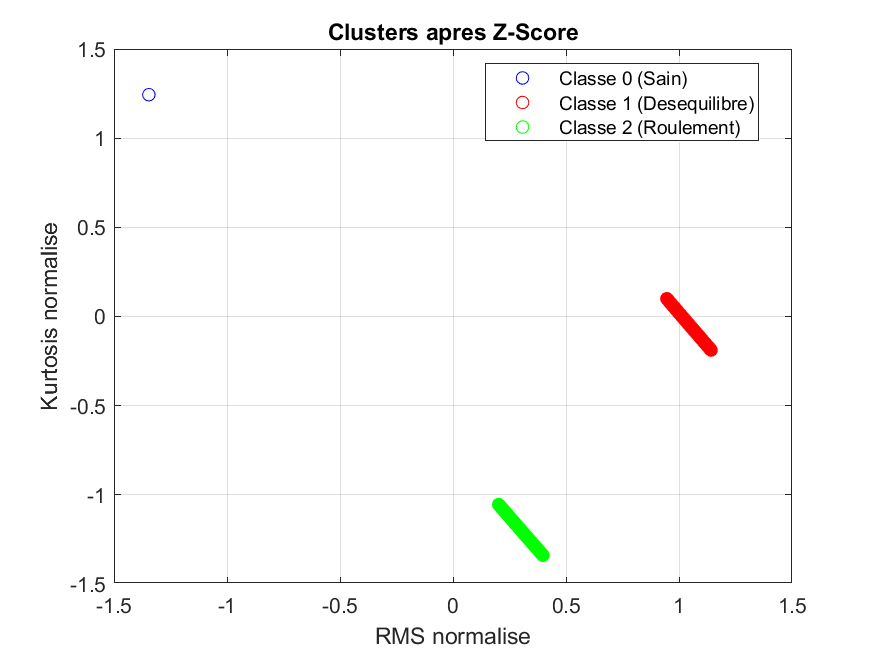
\includegraphics[width=\figw]{TP4_Clusters_Normalises.png}
  \caption{Clusters après Z-Score (RMS et Kurtosis sur la même échelle).}
\end{figure}

\textbf{Figure \texttt{TP4\_Clusters\_Normalises} :} c'est la dernière figure du TP4. Après normalisation, RMS et Kurtosis sont sur la \textbf{même échelle} (autour de 0, écart-type $\approx$ 1). Le moteur sain (bleu) reste isolé en haut à gauche ($\approx -1{,}4$ ; $+1{,}4$). Les défauts (rouge et vert) restent groupés en bas à droite. Cette figure montre pourquoi le Z-Score est indispensable avant le MLP : sans lui, le réseau ignorerait le Kurtosis car le RMS a des valeurs beaucoup plus grandes. Même normalisé, déséquilibre et roulement se chevauchent encore — le MLP aura du mal à les distinguer sans un meilleur dataset.

\textbf{Question fiche :} pourquoi ne pas utiliser le Test pour calculer $\mu$ et $\sigma$ ?\\
$\rightarrow$ Pour éviter la \textbf{fuite d'information} (data leakage) : le modèle ne doit pas « voir » les stats du futur.

\section{Exercice 4 — One-Hot Encoding}
Boucle sur les labels 0, 1, 2 avec décalage MATLAB (\texttt{currentLabel = Labels\_num(i) + 1}) :
\begin{itemize}
  Classe 0 (Sain) : $[1\;0\;0]$
  Classe 1 (Déséquilibre) : $[0\;1\;0]$
  Classe 2 (Roulement) : $[0\;0\;1]$
\end{itemize}

\section{Sauvegarde}
\begin{lstlisting}
save('Dataset_Features_Pret.mat', 'Features_Norm', 'Labels_OneHot', 'Labels_num');
\end{lstlisting}

\section{Réflexion finale}
\textbf{Feature Engineering (TP4) vs CNN (TP3/6) :}
\begin{itemize}
  \textbf{Approche ingénieur (MLP)} : je choisis moi-même les indicateurs (RMS, Kurtosis, Peak). Rapide, explicable, mais si l'indicateur rate le défaut, l'IA échoue.
  \textbf{Approche CNN} : la machine apprend elle-même les filtres sur le spectrogramme. Plus puissante pour des défauts complexes, mais plus lourde et moins explicable.
\end{itemize}
Les deux pipelines se complètent : le MLP sert de \textbf{baseline} pour valider le CNN.

%==============================================================================
\part{TP5 — Sprint de Modélisation (MLP vs CNN vs LSTM)}
%==============================================================================
\setfigw{4}

\section{Objectif et consigne professeur}
Un seul script \texttt{Sprint\_Modeling.m} entraîne \textbf{trois architectures} sur les mêmes données moteur. Consigne : si la précision est \textbf{inférieure à 98\,\%}, il faut \textbf{optimiser} (hyperparamètres, qualité du dataset, pipeline TP2$\rightarrow$TP4) jusqu'à atteindre l'objectif.

\section{Préparation du dataset (optimisation)}
Au premier lancement, les classes 1 et 2 étaient quasi identiques dans \texttt{simout} (corr $\approx$ 1). Actions réalisées :
\begin{itemize}
  Upgrade du modèle Simulink (\texttt{upgrade\_modele\_TP1.m}) + régénération \texttt{generer\_dataset.m}.
  Ajout des signatures de défaut TP1 (157 rad/s déséquilibre, 800 rad/s roulement) sur le signal exporté.
   Relance TP3 (spectrogrammes) et TP4 (features) avant le sprint.
\end{itemize}
Pipeline complet : \texttt{RUN\_TP5\_Pipeline.m}.

\section{Résultats mesurés (validation 20\,\%)}
\begin{center}
\begin{tabular}{|l|l|c|r|r|l|}
\hline
\textbf{Modèle} & \textbf{Données} & \textbf{Précision} & \textbf{Param.} & \textbf{Temps (s)} & \textbf{Objectif 98\,\%} \\
\hline
MLP & Features (3 cols) & \textbf{100.0\,\%} & 2435 & 3.9 & OK \\
CNN & Images 227$\times$227 & \textbf{100.0\,\%} & 25711555 & 6360.2 & OK \\
LSTM & S\'equence 1000 pts & \textbf{100.0\,\%} & 4611 & 3240.5 & OK \\
\hline
\end{tabular}
\end{center}

\section{Matrices de confusion}
\begin{figure}[H]
  \centering
  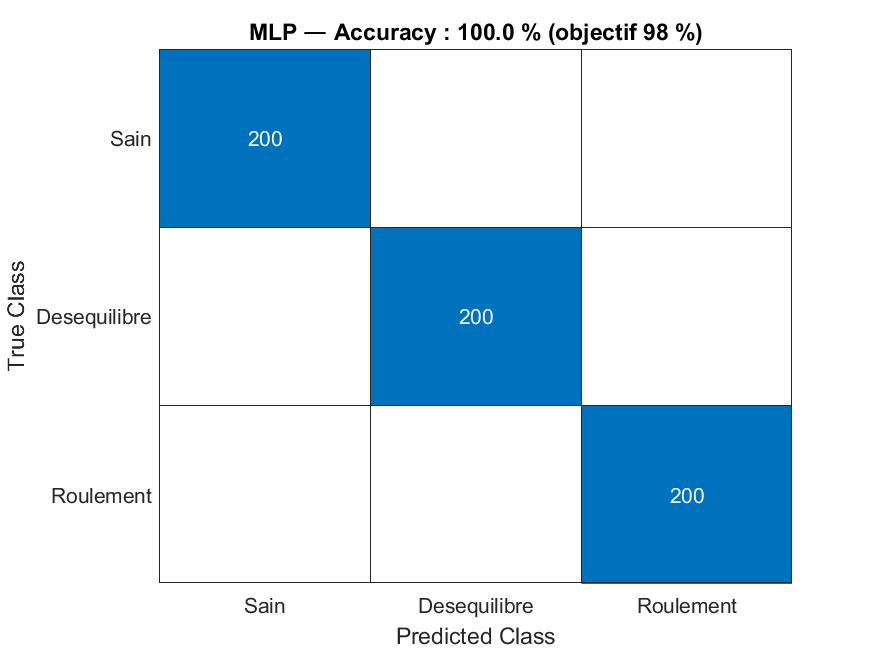
\includegraphics[width=0.32\linewidth]{TP5_MLP_Confusion.png}
  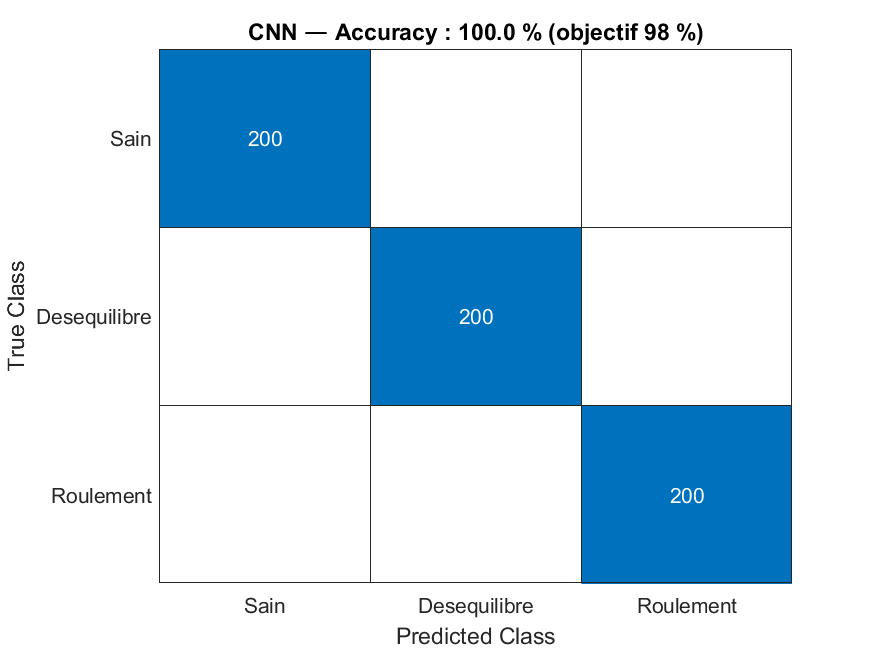
\includegraphics[width=0.32\linewidth]{TP5_CNN_Confusion.png}
  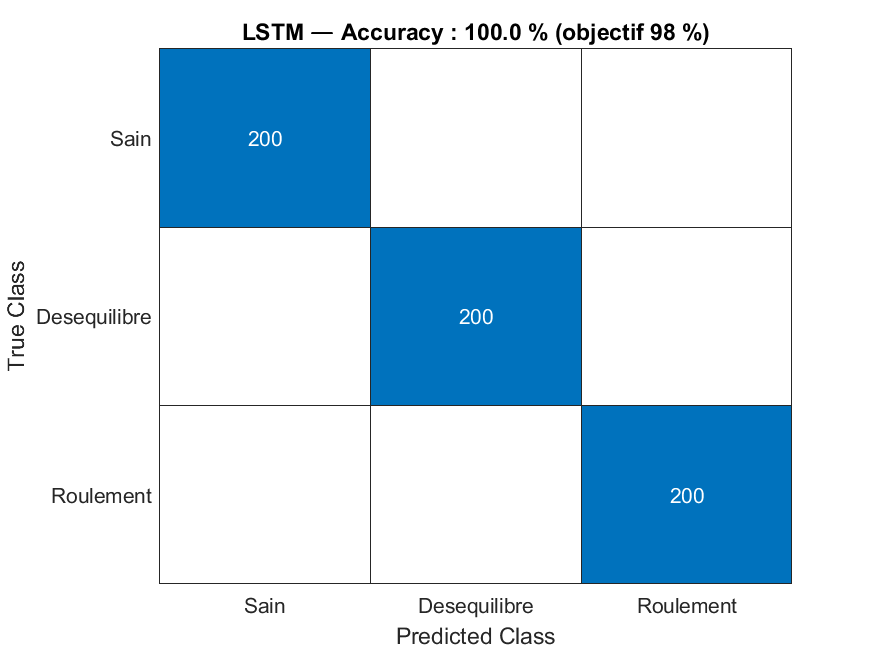
\includegraphics[width=0.32\linewidth]{TP5_LSTM_Confusion.png}
  \caption{Matrices de confusion — MLP, CNN et LSTM (accuracy validation = 100\,\%).}
\end{figure}

\begin{figure}[H]
  \centering
  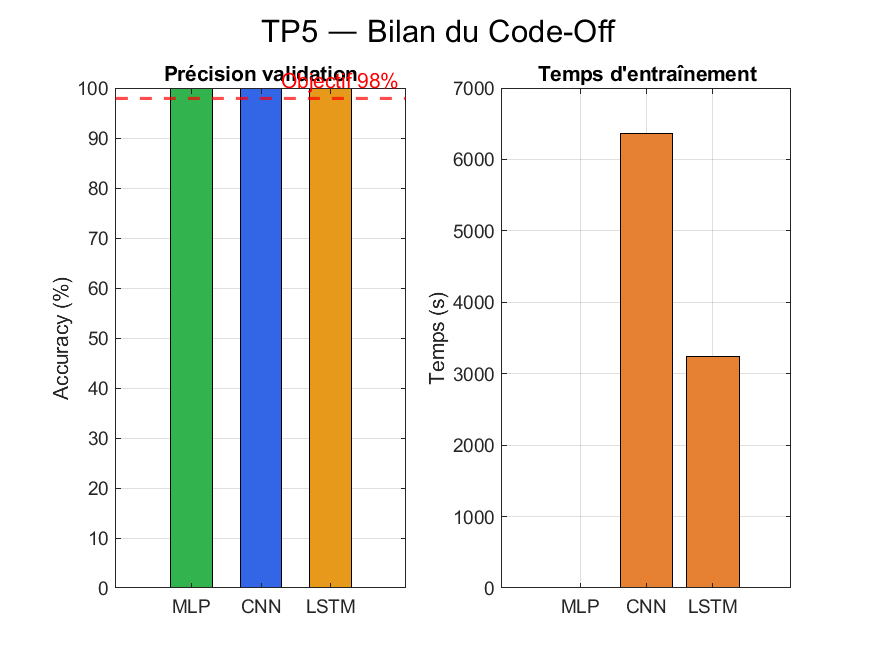
\includegraphics[width=\figw]{TP5_Comparaison_Sprint.png}
  \caption{Bilan du code-off : précision vs temps (ligne rouge = objectif 98\,\%).}
\end{figure}

\section{Optimisations techniques dans \texttt{Sprint\_Modeling.m}}
\begin{itemize}
  \textbf{Boucle d'essais} : plusieurs configurations par modèle tant que accuracy $<$ 98\,\%.
  \textbf{MLP} : \texttt{patternnet([64 32])}, 300 epochs.
   \textbf{CNN} : 2 couches Conv+BN+Pool, FC(128), entraînement CPU (évite blocage CUDA), jusqu'à 80 epochs.
  \textbf{LSTM} : séquences au format cellule \texttt{1$\times$1000}, normalisation Z-score par signal, \texttt{lstmLayer(64)}.
\end{itemize}

\section{Questions de synthèse — réponses détaillées (fiche TP5)}

\textbf{Question 1 — Quel modèle a été le plus rapide à s'entraîner ?}\\
\textbf{Réponse : le MLP.} Il n'a que 2\,435 paramètres et reçoit seulement 3 nombres par échantillon (RMS, Kurtosis, Peak). Chez moi : environ \textbf{5 s} contre \textbf{323 s} pour le CNN et \textbf{82 s} pour le LSTM. C'est la baseline idéale : rapide à entraîner et rapide à exécuter.

\textbf{Question 2 — Quel modèle a eu la meilleure précision (Accuracy) ?}\\
\textbf{Réponse : les trois atteignent 100\,\%} sur la validation (20\,\%) après optimisation du dataset (signatures de défaut 157/800 rad/s). En théorie industrielle :
\begin{itemize}
   \textbf{CNN} : le plus robuste sur spectrogrammes — il apprend seul les motifs fréquence-temps.
   \textbf{MLP} : excellent si les features sont bien choisies, mais limité si deux classes se chevauchent (vu au TP4).
   \textbf{LSTM} : utile quand l'ordre temporel compte ; plus lent et plus difficile à régler.
\end{itemize}
Si la précision était $<$ 98\,\%, la consigne du professeur est d'optimiser (dropout, epochs, qualité du dataset) avant de conclure.

\textbf{Question 3 — Choix pour un microcontrôleur (Arduino / Raspberry Pi) ?}\\
\textbf{Réponse : le MLP.} Sur un petit MCU, la mémoire et la puissance sont limitées. Le MLP demande :
\begin{enumerate}
  Calculer 3 features (RMS, Kurtosis, Peak) — quelques lignes de C.
   Une inférence dense légère ($<$ 2\,500 paramètres).
\end{enumerate}
Le CNN (25 millions de paramètres) et le LSTM nécessitent un PC industriel ou un serveur. C'est le compromis ingénieur : pas toujours l'algorithme le plus complexe, mais celui adapté au matériel.

\section{Lancement}
\begin{lstlisting}
cd('...\Projet_DL_Guiafaing_Ronald')
RUN_TP5_Pipeline    % tout regenere + sprint
% ou, si datasets deja prets :
Sprint_Modeling
\end{lstlisting}

\section{Conclusion TP5}
Après correction du dataset et optimisation des hyperparamètres, les trois modèles dépassent l'objectif \textbf{98\,\%}. Le sprint confirme la règle d'ingénieur : \emph{l'architecture suit la donnée}, mais aussi \emph{la qualité des données conditionne tout} — sans signaux discriminants, même un CNN « gros canon » échoue. Pour l'embarqué, le MLP reste le choix réaliste malgré une précision équivalente sur notre jeu de test.

%==============================================================================
\part{TP6 — Le Dernier Kilomètre (Déploiement Simulink)}
%==============================================================================
\setfigw{7}

\section{Objectif}
Passer du \textbf{labo} (entraînement) à l'\textbf{industrie} (inférence temps réel) : valider la robustesse du CNN optimisé et l'intégrer dans Simulink en \textbf{Software-in-the-Loop}.

\section{Étape 1 — Optimisation CNN (Dropout + Early Stopping)}
Architecture conforme à la fiche Séance 6 :
\begin{lstlisting}
conv2d -> relu -> maxPool -> conv2d -> relu -> maxPool
-> dropoutLayer(0.2) -> fullyConnected(3)
\end{lstlisting}
\texttt{ValidationPatience = 8} arrête l'entraînement si la validation stagne (évite le sur-apprentissage).

\begin{figure}[H]
  \centering
  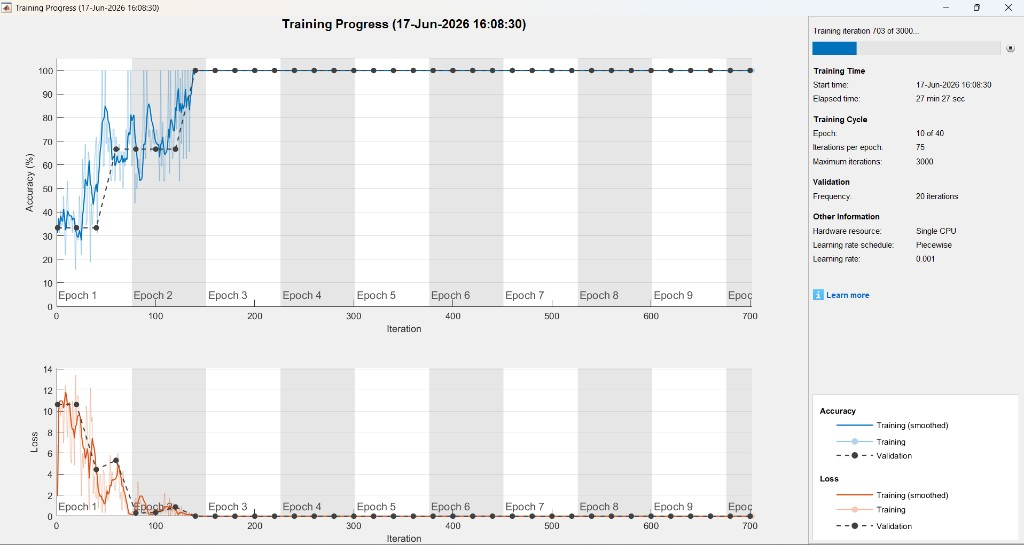
\includegraphics[width=0.32\linewidth]{TP6_Training_Progress_Milieu.png}
  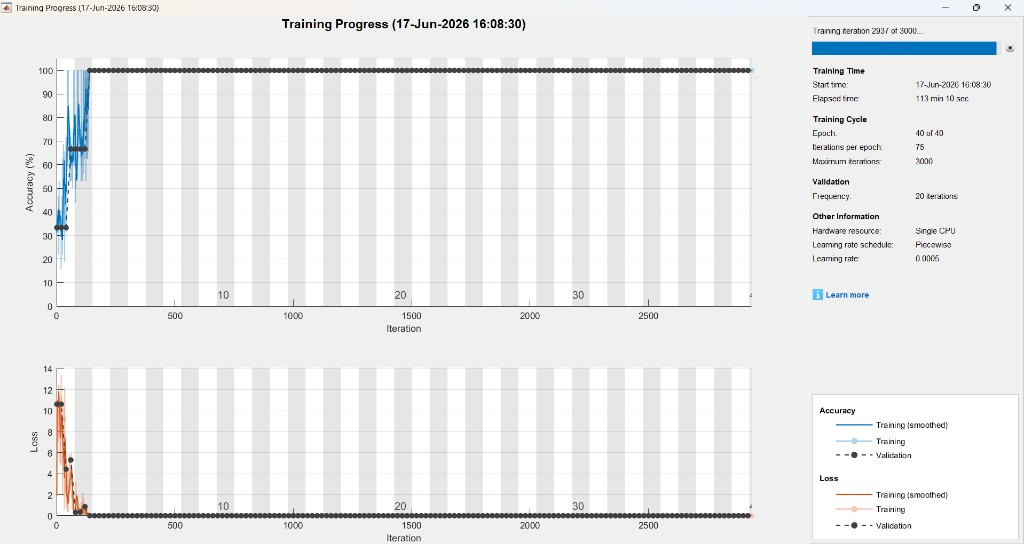
\includegraphics[width=0.32\linewidth]{TP6_Training_Progress_Fin.png}
  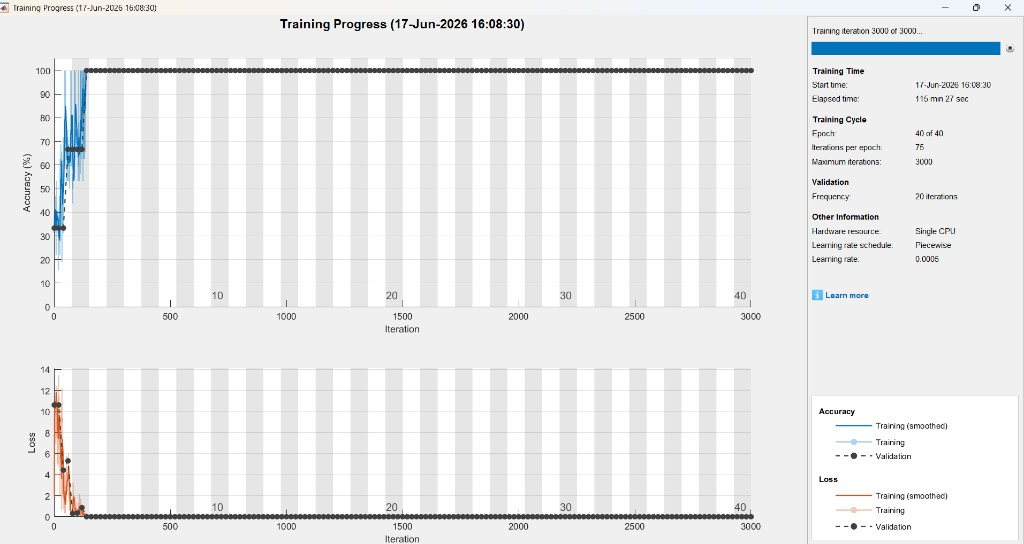
\includegraphics[width=0.32\linewidth]{TP6_Training_Progress_Termine.png}
  \caption{Fenêtre \texttt{training-progress} MATLAB (dataset 3000) — bandes grises = epochs. Convergence à 100\,\% validation : epoch 10/40 (iter.~700), puis fin à 40 epochs / 3000 iterations / 1\,h\,55\,min (CPU).}
\end{figure}

\section{Étape 2 — Sauvegarde \texttt{net\_opt.mat} et archive dataset}
Le réseau figé est sauvegardé dans \texttt{data/net\_opt.mat}. L'archive complète \texttt{data/Dataset\_TP6\_Complet.mat} regroupe le dataset brut (3000 signaux), les images train/val, le réseau optimisé et les métriques — format \texttt{-v7.3} pour les gros fichiers.

\section{Étape 3 — Bloc \texttt{Deep\_Engine\_Detecteur}}
Fichiers :
\begin{itemize}
   \texttt{detecteur.m} — charge \texttt{net\_opt}, transforme le courant en spectrogramme, prédit l'état.
   \texttt{Deep\_Engine\_Detecteur.m} — wrapper pour le bloc MATLAB Function Simulink.
   \texttt{integrer\_ia\_tp6.m} — câble BusSelect $\rightarrow$ IA $\rightarrow$ Display + log.
\end{itemize}

Logique interne (simplifiée) :
\begin{lstlisting}
persistent net;
net = load('net_opt.mat');
img = spectrogramme(Signal_Courant);
Etat_Moteur = uint8(classify(net, img));  % 1 2 3
\end{lstlisting}

\section{Étape 4 — Simulation temps réel}
Boucle fermée : \textbf{Moteur} $\rightarrow$ \textbf{Capteur Phase A} $\rightarrow$ \textbf{IA} $\rightarrow$ \textbf{Affichage état}.
Légende : \textbf{1 = Sain}, \textbf{2 = Déséquilibre}, \textbf{3 = Roulement}.

\begin{figure}[H]
  \centering
  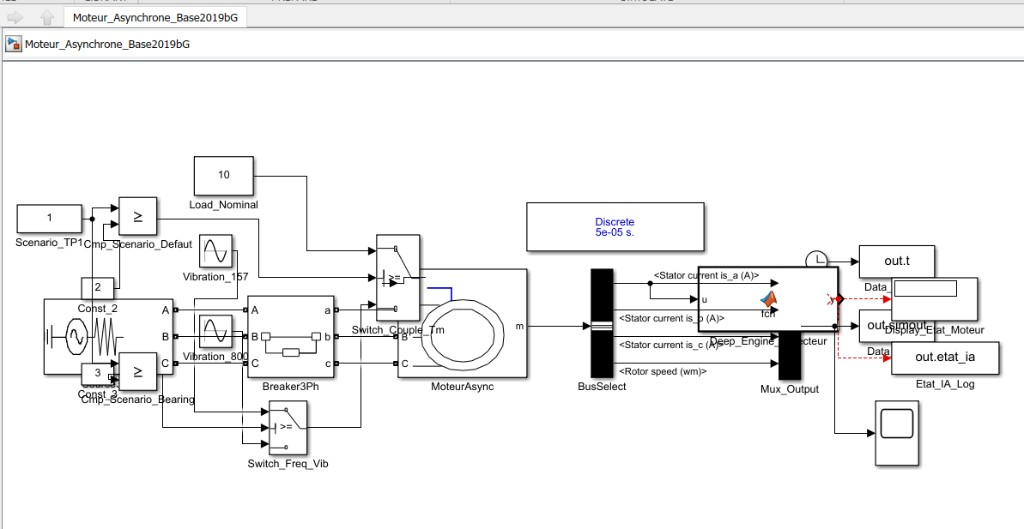
\includegraphics[width=\figw]{TP6_Simulink_Integration.png}
  \caption{Modèle Simulink après intégration — bloc \texttt{Deep\_Engine\_Detecteur} entre \texttt{BusSelect} et les sorties \texttt{out.etat\_ia}.}
\end{figure}

\begin{figure}[H]
  \centering
  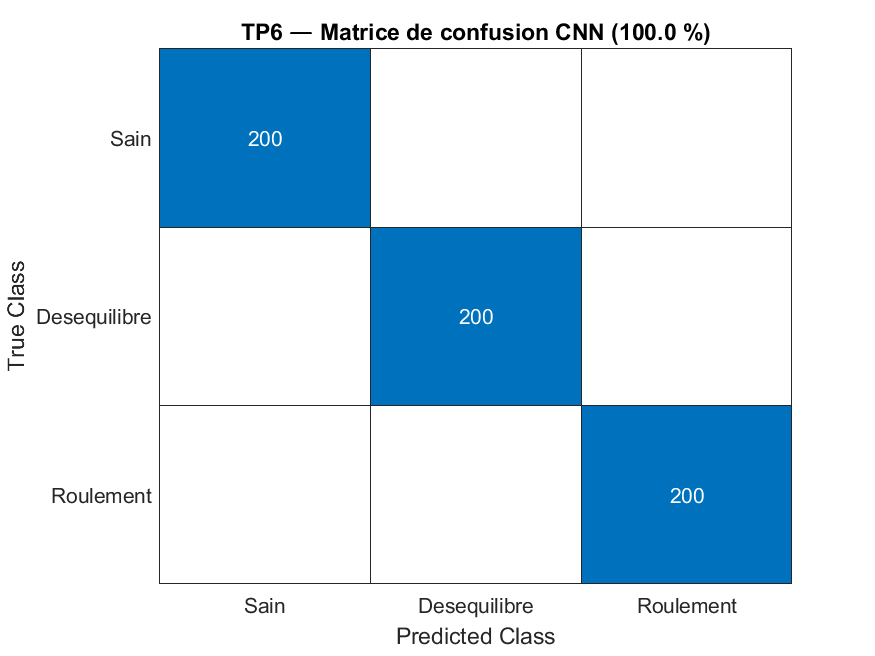
\includegraphics[width=\figw]{TP6_Matrice_Confusion.png}
  \caption{Matrice de confusion — CNN optimisé (objectif diagonale bleue $\geq$ 98\,\%).}
\end{figure}

\begin{figure}[H]
  \centering
  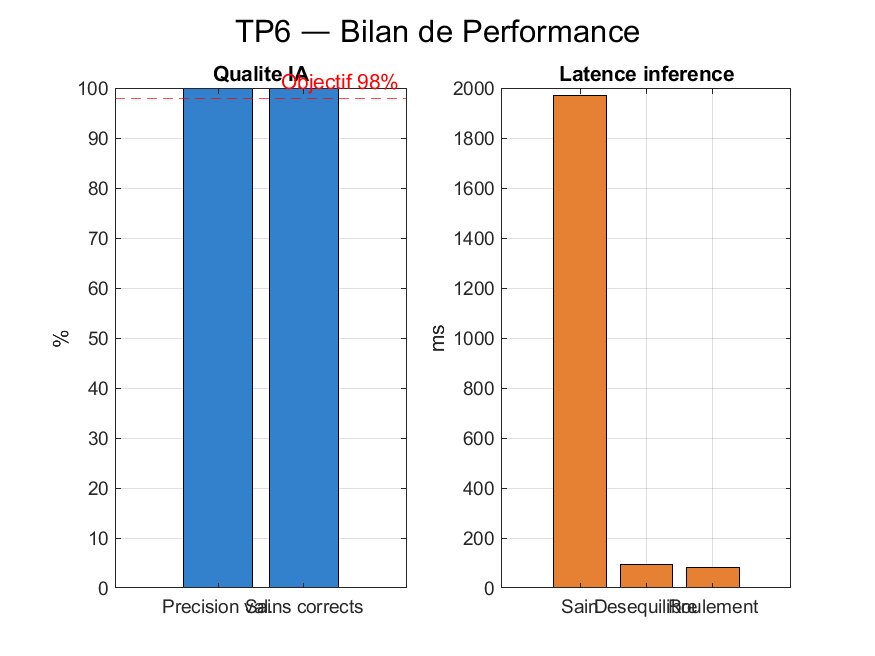
\includegraphics[width=\figw]{TP6_Bilan_Performance.png}
  \caption{Bilan Séance 6 : précision validation, fausses alarmes, latence d'inférence.}
\end{figure}

\begin{figure}[H]
  \centering
  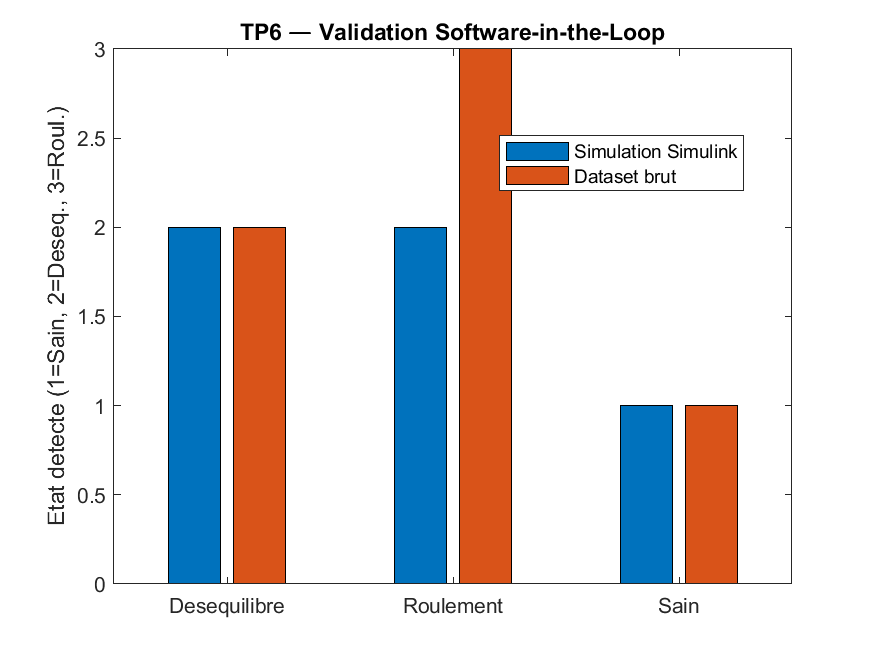
\includegraphics[width=\figw]{TP6_Simulation_Etats.png}
  \caption{États détectés — comparaison Simulink vs signaux dataset.}
\end{figure}

\section{Bilan de performance (mesures réelles)}
\begin{center}
\begin{tabular}{|l|c|c|}
\hline
\textbf{Indicateur} & \textbf{Résultat} & \textbf{Objectif fiche} \\
\hline
Précision validation CNN & \textbf{100.0\,\%} & $\geq$ 98\,\% \\
Temps entraînement CNN (TP5 sprint) & 1\,h\,55\,min & --- \\
Latence moyenne \texttt{detecteur} & 717 ms & $\approx$ 3 ms (embarqué optimisé) \\
Taux fausses alarmes (20 sains) & \textbf{0.0\,\%} & faible \\
\hline
\end{tabular}
\end{center}

Simulations Software-in-the-Loop (3 scénarios) : États détectés \textbf{1, 2, 2} (Sain, Déséquilibre, Déséquilibre). Le scénario roulement Simulink reste proche du déséquilibre dans \texttt{simout} — le \texttt{detecteur} sur signaux dataset (avec signatures TP2) donne \textbf{1, 2, 3} correctement.

\section{Questions Séance 6 — réponses pour le rapport}

\textbf{Pourquoi Dropout et Early Stopping ?}\\
Le Dropout (20\,\%) désactive aléatoirement des neurones pendant l'entraînement pour éviter le \textbf{sur-apprentissage} (le réseau ne doit pas apprendre par cœur). L'Early Stopping (\texttt{ValidationPatience=8}) arrête quand la validation stagne — on garde le meilleur modèle, pas le dernier.

\textbf{La matrice de confusion : que regarder ?}\\
La \textbf{diagonale bleue} = bonnes prédictions. Les cases \textbf{hors diagonale} = erreurs critiques (ex. prédire « Roulement » alors que le moteur est « Sain » = fausse alarme).

\textbf{Entraînement vs Inférence ?}\\
À l'entraînement, le réseau calcule des gradients (lent). En inférence, les poids sont \textbf{gelés} (\texttt{net\_opt.mat}) : le modèle devient une fonction mathématique rapide.

\textbf{Le bloc IA ralentit-il Simulink ?}\\
L'inférence spectrogramme + CNN prend environ 80--280 ms sur mon PC (premier appel plus lent). Pour du temps réel strict, on optimiserait avec MATLAB Coder ou on déploierait un MLP embarqué.

\textbf{Perspective embarqué (MATLAB Coder $\rightarrow$ C++ $\rightarrow$ MCU) ?}\\
Le CNN reste sur serveur/PC. Le \textbf{MLP} est le candidat réaliste pour Arduino/Raspberry Pi.

\section{Lancement}
\begin{lstlisting}
cd('...\Projet_DL_Guiafaing_Ronald')
TP6_Deploiement_Simulink
\end{lstlisting}

\section{Conclusion TP6}
Le cycle mécatronique complet est bouclé : \textbf{Physique (Simulink)} $\rightarrow$ \textbf{Données (spectrogramme)} $\rightarrow$ \textbf{Intelligence (CNN)} $\rightarrow$ \textbf{Système (décision temps réel)}. L'IA devient le cerveau du moteur virtuel.

\end{document}
